\section{Experiment Details}\label{supp:details}


\subsection{Experimental Setup}\label{supp:exp_details}

\textbf{Domains.} We provide a breakdown of the number of tokens per domain in Table~\ref{tab:domain_sizes}.

\begin{table}[h]
\centering
\caption{Token counts for all domains in the final domain set. Sources with topic-level partitions (DCLM, Stack-Edu, olmOCR Science PDFs) are shown with indented topics. Single-source domains are shown without subdivision.}
\small
\begin{tabular}{l r | l r}
\toprule
\textbf{Domain} & \textbf{Token Count} & \textbf{Domain} & \textbf{Token Count} \\
\midrule
\multicolumn{2}{l|}{\textbf{DCLM}~\citep{dclm}} & \multicolumn{2}{l}{\textbf{Stack-Edu}~\citep{allal2025smollm2smolgoesbig}} \\
\quad Adult Content & 67,760,078,203 & \quad C & 4,735,074,247 \\
\quad Art and Design & 70,659,711,995 & \quad C\# & 7,204,525,343 \\
\quad Crime and Law & 170,130,914,779 & \quad C++ & 12,530,445,761 \\
\quad Education and Jobs & 184,690,792,861 & \quad Go & 1,398,595,118 \\
\quad Electronics and Hardware & 80,168,541,745 & \quad Java & 31,347,725,888 \\
\quad Entertainment & 441,768,061,760 & \quad JavaScript & 8,886,972,357 \\
\quad Fashion and Beauty & 37,256,539,512 & \quad Markdown & 28,916,320,218 \\
\quad Finance and Business & 310,313,927,581 & \quad PHP & 7,395,033,318 \\
\quad Food and Dining & 105,937,299,687 & \quad Python & 18,017,832,560 \\
\quad Games & 229,992,491,702 & \quad Ruby & 1,386,775,805 \\
\quad Health & 393,496,227,836 & \quad Rust & 1,418,447,132 \\
\quad History and Geography & 161,049,719,459 & \quad SQL & 7,063,472,860 \\
\quad Home and Hobbies & 126,910,777,314 & \quad Shell & 2,542,637,875 \\
\quad Industrial & 43,572,140,450 & \quad Swift & 1,510,019,025 \\
\quad Literature & 364,834,344,848 & \quad TypeScript & 2,495,753,789 \\
\quad Politics & 611,198,130,192 & \multicolumn{2}{l}{} \\
\quad Religion & 277,776,929,208 & \multicolumn{2}{l}{\textbf{olmOCR Science PDFs}~\citep{olmo2025olmo3}} \\
\quad Science, Math and Technology & 427,131,054,341 & \quad Adult & 303,073,226 \\
\quad Social Life & 218,731,841,124 & \quad Art and Design & 6,833,185,034 \\
\quad Software & 108,039,380,021 & \quad Crime and Law & 42,538,674,743 \\
\quad Software Development & 223,384,974,282 & \quad Education and Jobs & 138,127,926,093 \\
\quad Sports and Fitness & 196,759,999,355 & \quad Entertainment & 6,069,602,783 \\
\quad Transportation & 90,793,306,202 & \quad Fashion and Beauty & 557,917,820 \\
\quad Travel and Tourism & 57,642,815,530 & \quad Finance and Business & 61,150,044,703 \\
 & & \quad Food and Dining & 2,322,982,204 \\
\multicolumn{2}{l|}{\textbf{Single-Source Domains}} & \quad Games & 2,486,095,532 \\
\textbf{AlgebraicStack}~\citep{azerbayev2023llemma} & 11,818,955,329 & \quad Health & 108,215,933,374 \\
\textbf{ArXiv}~\citep{azerbayev2023llemma} & 20,773,846,846 & \quad Home and Hobbies & 3,924,579,643 \\
\textbf{FineMath-3+}~\citep{allal2025smollm2smolgoesbig} & 34,057,973,953 & \quad Industrial & 29,389,278,657 \\
\textbf{Pes2o}~\citep{peS2o} & 58,552,461,187 & \quad Literature & 31,886,391,090 \\
\textbf{Wikipedia}~\citep{soldaini2024dolma} & 10,067,758,073 & \quad Politics & 39,234,116,889 \\
 & & \quad Religion & 24,729,732,953 \\
 & & \quad Science and Technology & 424,245,385,160 \\
 & & \quad Software & 9,146,853,216 \\
 & & \quad Software Development & 41,841,278,724 \\
 & & \quad Sports and Fitness & 5,450,913,796 \\
 & & \quad Transportation & 17,149,342,957 \\
 & & \quad Travel & 2,102,425,717 \\
\bottomrule
\end{tabular}
\label{tab:domain_sizes}
\end{table}




\textbf{Model.} We train 1B parameter decoder-only transformer models using Olmo 2 architecture~\citep{olmo20242olmo2furious}. In particular, we set n\_layers=16, n\_head=16, d\_model=2048, head\_dim=128.

We use a batch size of 512, a learning rate of $0.0018$ with a cosine scheduler with warmup and linear decay, and a sequence length of 4096. We use the Dolma 2 tokenizer.

All 1B models were trained on 32 NVIDIA H100s (80 GB), while proxy models were trained on one NVIDIA H100. 


\textbf{Evaluation.} Table~\ref{tab:eval_suite} lists all the downstream tasks. 

\begin{table}[t]
  \centering
  \caption{
  \textbf{Details of the BPB evaluation suite}. 
  We use the \textsc{OlmoBaseEval} easy evaluation suite \citep{olmo2025olmo3}, formatted as bits-per-byte (BPB) over gold continuations. $^\dagger$ = few-shot examples are built-in the task; $^\alpha$ = human-written few-shot examples. We treat subtasks as standalone tasks, except for MMLU, where we use averages over the four MMLU categories. 
  }
\begin{scriptsize}
\begin{tabular}{lllccc}
\toprule
& \bf{Task} & \bf{Capability} & \bf{\# ICL} & \bf{Metric} & \bf{\# Subtasks} \\
\midrule

\rowcolor{ai2offwhite} & Minerva MATH (\citeyear{lewkowycz2022solving}) & Math Gen & 4$^\alpha$ & BPB & 7 \\
\rowcolor{ai2offwhite} & \multicolumn{5}{l}{\hspace{6pt}Subtasks: \textit{Algebra, Counting and Probability, Geometry, Intermediate Algebra} } \\
\rowcolor{ai2offwhite}\rowcolor{ai2offwhite} \multirow{-3}{*}{\rotatebox[origin=c]{90}{\textit{Math}}} & \multicolumn{5}{l}{\hspace{6pt}\textit{Number Theory, Prealgebra, Precalculus} } \\
\rowcolor{lightgrey} & HumanEval (\citeyear{chen2021codex}) & Code Gen & 3 & BPB & - \\
\rowcolor{lightgrey} & MBPP (\citeyear{austin2021program}) & Code Gen & 3 & BPB & - \\
\rowcolor{lightgrey} & MT MBPP (\citeyear{cassano2022multipl, olmo2025olmo3}) & Code Gen & 3 & BPB & 17 \\
\rowcolor{lightgrey} & \multicolumn{5}{l}{\hspace{6pt}Subtasks: \textit{Bash, C, C++, C\#, Go, Haskell, Java, JavaScript, MatLab, PHP} } \\
\rowcolor{lightgrey}\multirow{-5}{*}{\rotatebox[origin=c]{90}{\textit{Code}}} & \multicolumn{5}{l}{\hspace{6pt}\textit{Python, R, Ruby, Rust, Scala, Swift, TypeScript} } \\
\rowcolor{ai2offwhite} & ARC (\citeyear{clark2018think}) & Science QA & 5 & BPB & 2 \\
\rowcolor{ai2offwhite} & \multicolumn{5}{l}{\hspace{6pt}Subtasks: \textit{ARC-Easy, ARC-Challenge} } \\
\rowcolor{ai2offwhite} & MMLU STEM (\citeyear{hendryckstest2021}) & General QA & 5 & BPB & 19 \\
\rowcolor{ai2offwhite} & MMLU Humanities (\citeyear{hendryckstest2021}) & General QA & 5 & BPB & 13 \\
\rowcolor{ai2offwhite} & MMLU Social Sci. (\citeyear{hendryckstest2021}) & General QA & 5 & BPB & 12 \\
\rowcolor{ai2offwhite} & MMLU Other (\citeyear{hendryckstest2021}) & General QA & 5 & BPB & 14 \\
\rowcolor{ai2offwhite} & CSQA (\citeyear{talmor-etal-2019-commonsenseqa}) & Commonsense QA & 5 & BPB & - \\
\rowcolor{ai2offwhite} & HellaSwag (\citeyear{zellers-etal-2019-hellaswag}) & Language Modeling & 5 & BPB & - \\
\rowcolor{ai2offwhite} & WinoGrande (\citeyear{Sakaguchi_Le_Bras_Bhagavatula_Choi_2020}) & Language Modeling & 5 & BPB & - \\
\rowcolor{ai2offwhite} & SocialIQA (\citeyear{sap-etal-2019-social}) & Social QA & 5 & BPB & - \\
\rowcolor{ai2offwhite} & PiQA (\citeyear{Bisk_Zellers_Le_bras_Gao_Choi_2020}) & Physical QA & 5 & BPB & - \\
\rowcolor{ai2offwhite} & CoQA (\citeyear{reddy-etal-2019-coqa}) & Conversation QA & 0$^\dagger$ & BPB & - \\
\rowcolor{ai2offwhite} & DROP (\citeyear{dua-etal-2019-drop}) & Passage QA & 5 & BPB & - \\
\rowcolor{ai2offwhite} & Jeopardy (\citeyear{mosaic-jeopardy}) & Trivia QA & 5 & BPB & - \\
\rowcolor{ai2offwhite} & NaturalQs (\citeyear{kwiatkowski-etal-2019-natural}) & General QA & 5 & BPB & - \\
\rowcolor{ai2offwhite} & SQuAD (\citeyear{rajpurkar-etal-2016-squad}) & General QA & 5 & BPB & - \\
\rowcolor{ai2offwhite} & SciQ (\citeyear{welbl-etal-2017-crowdsourcing}) & Science QA & 5 & BPB & - \\
\rowcolor{ai2offwhite} & Basic Skills (\citeyear{olmo2025olmo3}) & Basic QA & 5 & BPB & 6 \\
\rowcolor{ai2offwhite} & \multicolumn{5}{l}{\hspace{6pt}Subtasks: \textit{Basic Arithmetic, String Manipulation, Simple Coding} } \\
\rowcolor{ai2offwhite} & \multicolumn{5}{l}{\hspace{6pt}\textit{Elementary Logical Reasoning, Basic Common Sense, Simple Pattern Recognition} } \\
\rowcolor{ai2offwhite} & Lambada (\citeyear{paperno2016lambada}) & Language Modeling & 0 & BPB & - \\
\rowcolor{ai2offwhite} \multirow{-23}{*}{\rotatebox[origin=c]{90}{\textit{QA}}} & MedMCQA (\citeyear{pmlr-v174-pal22a}) & Medical QA & 5 & BPB & - \\
\bottomrule
\end{tabular}
\end{scriptsize}
  \vspace{6pt}
  \label{tab:eval_suite}
\end{table}




\subsection{Implementation Details}\label{supp:imp_details}

For \fullmixreuse and \partialmixreuse, the first $\tilde{p}$ is from applying \base on the initial web corpus. After each update, the newly recomputed mix becomes the $\tilde{p}$ of the next one.


Across all swarm-based methods we evaluate on (\base, Swarm Reuse, \fullmixreuse, \partialmixreuse), we use $\Ssmall=30$M parameters (architecture in Table~\ref{tab:model_architectures}) and train for 5x Chinchilla, with a batch size of 64, a learning rate of $0.007$, and a sequence length of 2048. 

For any $m$ domains we want to recompute, we set $K$ to approximate $c(m + 1)$ for linear multiplier $c = 1, 2, 3$. In particular, for $c = 3$, we set $K = 2^x$ to be the power of $2$ that is closest to $3(m+1)$. For $c = 2$, we set $K = 2^{x-1}$. For $c = 1$, we set $K = m+1$. When we recompute over $m=2$ domains, we use search instead of regression, as the search space is one-dimensional. See Tables~\ref{tab:cost_fullrecomputation}, \ref{tab:cost_swarmreuse}, \ref{tab:cost_fullreuse}, and~\ref{tab:cost_partialreuse} for exact swarm sizes.
We solve all of our mixture optimization problems using CVXPY and a KL regularization term with $\lambda=0.05$. We set $k=4$ and $R = 1$T for the repetition constraint of the experiments in \S\ref{sec:superswarm}. 


\begin{table}[!h]
\centering
\caption{Swarm details per stage for \textbf{Full Recomputation}. We list the number of domains recomputed at each stage, and the columns with $c$ contain the number of proxy runs $K \approx c(m+1)$.}
\footnotesize
\setlength{\tabcolsep}{6pt}
\begin{tabular}{lcccc}
\toprule
\textbf{Stage} & \textbf{\# domains recomputed} & \textbf{$c=1$} & \textbf{$c=2$} & \textbf{$c=3$} \\
\midrule
Initial      & 24 & 25 & 32 & 64 \\
\Add (Stack-Edu languages)  & 39 & 40 & 64 & 128 \\
\Add (ArXiv, FineMath 3+, PDFs, Wiki, AlgebraicStack, pes2o) & 45 & 46 & 64 & 128 \\
\Revise (PDFs) & 45 & 46 & 64 & 128 \\
\Remove (AlgebraicStack) & 44 & 45 & 64 & 128 \\
\Partition (PDFs) & 64 & 65 & 128 & 256 \\
\midrule
\textbf{Total \# proxy runs} & & 267 & 416 & 832 \\
\bottomrule
\end{tabular}
\label{tab:cost_fullrecomputation}
\end{table}

\begin{table}[!h]
\centering
\caption{Swarm details per stage for \textbf{Swarm Reuse}. We list the number of domains recomputed at each stage, and the columns with $c$ contain the number of additional proxy runs needed, $K \approx c(m+1)$. $c=3$ corresponds to Figure~\ref{fig:main_results}.}
\footnotesize
\setlength{\tabcolsep}{6pt}
\begin{tabular}{lcccc}
\toprule
\textbf{Stage} & \textbf{\# domains recomputed} & \textbf{$c=1$} & \textbf{$c=2$} & \textbf{$c=3$} \\
\midrule
Initial      & 24 & 25 & 32 & 64 \\
\Add (Stack-Edu languages)  & 39 & 15 & 32 & 64 \\
\Add (ArXiv, FineMath 3+, PDFs, Wiki, AlgebraicStack, pes2o) & 45 & 6 & 6 & 6 \\
\Revise (PDFs) & 45 & 6 & 6 & 6 \\
\Remove (AlgebraicStack) & 44 & 5 & 5 & 5 \\
\Partition (PDFs) & 64 & 20 & 59 & 123 \\
\midrule
\textbf{Total \# proxy runs} & & 77 & 140 & 268 \\
\bottomrule
\end{tabular}
\label{tab:cost_swarmreuse}
\end{table}


\begin{table}[!h]
\centering
\caption{Swarm details per stage for \textbf{Full Mixture Reuse}. We list the number of domains recomputed at each stage, and the columns with $c$ contain the number of proxy runs $K \approx c(m+1)$. $c=3$ corresponds to Figure~\ref{fig:main_results}.}
\footnotesize
\setlength{\tabcolsep}{6pt}
\begin{tabular}{lcccc}
\toprule
\textbf{Stage} & \textbf{\# domains recomputed} & \textbf{$c=1$} & \textbf{$c=2$} & \textbf{$c=3$} \\
\midrule
Initial      & 24 & 25 & 32 & 64 \\
\Add (Stack-Edu languages)  & 16 & 17 & 32 & 64 \\
\Add (ArXiv, FineMath 3+, PDFs, Wiki, AlgebraicStack, pes2o) & 7 & 8 & 8 & 16 \\
\Revise (PDFs) & 2 & 3 & 4 & 8 \\
\Remove (AlgebraicStack) & 0 & 0 & 0 & 0 \\
\Partition (PDFs) & 22 & 23 & 32 & 64 \\
\midrule
\textbf{Total \# proxy runs} &  & 76 & 108 & 216 \\
\bottomrule
\end{tabular}
\label{tab:cost_fullreuse}
\end{table}

\begin{table}[!h]
\centering
\caption{Swarm details per stage for \textbf{Partial Mixture Reuse}. We list the number of domains recomputed at each stage, and the columns with $c$ contain the number of proxy runs $K \approx c(m+1)$. $c=3$ corresponds to Figure~\ref{fig:main_results}.}
\footnotesize
\setlength{\tabcolsep}{6pt}
\begin{tabular}{lcc}
\toprule
\textbf{Stage} & \textbf{\# domains ($m$)} & \textbf{Proxy Runs ($c=3$)} \\
\midrule
Initial      & 24 & 64 \\
\Add (Stack-Edu languages)  & 17 & 64 \\
\Add (ArXiv, FineMath 3+, PDFs, Wiki, AlgebraicStack, pes2o) & 8 & 32 \\
\Revise (PDFs) & 8 & 32 \\
\Remove (AlgebraicStack) & 7 & 16 \\
\Partition (PDFs) & 27 & 64 \\
\midrule
\textbf{Total \# proxy runs} &  & 272 \\
\bottomrule
\end{tabular}
\label{tab:cost_partialreuse}
\end{table}





Algorithm~\ref{alg:swarm_reuse_method} corresponds to the Swarm Reuse approach in \S\ref{sec:superswarm}, presenting another way to reuse prior information from mixing. 
The blue coloring indicates aspects of this algorithm that are different from \base. 


\begin{algorithm}[htb]
   \caption{Swarm Reuse Mixing}
   \label{alg:swarm_reuse_method}
\begin{algorithmic}[1]
   \STATE {\bfseries Input:} \textcolor{olmoBlue}{Old domain set $\D$, new domain set $\D'$, old swarm $\{(p^j_{\text{old}}, \{y_{ij}^{\text{old}}\}_{i=1}^n)\}_{j=1}^{K_{\text{old}}}$}, new swarm size $K_{\text{new}} = \mathcal{O}(|\D'|)$, Dirichlet distribution $\mathcal{P}'$, repetition factor $k$, requested tokens $R$.
   \STATE Sample new mixes $p^1_{\text{new}}, \dots, p^{K_{\text{new}}}_{\text{new}} \sim \mathcal{P}'$ on $\D'$.
   \STATE Train proxy models on new mixes and evaluate on downstream tasks to get new swarm data $\{(p^j_{\text{new}}, \{y_{ij}^{\text{new}}\}_{i = 1}^n \}_{j =1}^{K_{\text{new}}}$.
   \STATE \textcolor{olmoBlue}{Map old swarm mixes to new domain set: for $j \in [K_{\text{old}}]$, compute $\tilde{p}^j_{\text{old}} \in \triangle^{m'-1}$ from $p^j_{\text{old}} \in \triangle^{m-1}$ where:}
   \begin{itemize}
       \item \textcolor{olmoBlue}{If \textbf{Add}: $\D = [\D_1, \emptyset]$ and $\D' = [\D_1, \D_2']$. Then $\tilde{p}^j_{\text{old}}(D_i') = p^j_{\text{old}}(D_i)$ for $D_i \in \D_1$, and $\tilde{p}^j_{\text{old}}(D_i') = 0$ for $D_i' \in \D_2'$.}
       \item \textcolor{olmoBlue}{If \textbf{Partition}: $\D = [\D_1, \{D_{\text{par}}\}]$ and $\D' = [\D_1, \{D_{\text{par}}^1, \dots, D_{\text{par}}^{\ell}\}]$ where $D_{\text{par}} = \bigcup_{k=1}^{\ell} D_{\text{par}}^k$. Then $\tilde{p}^j_{\text{old}}(D_i') = p^j_{\text{old}}(D_i)$ for $D_i \in \D_1$, and $\tilde{p}^j_{\text{old}}(D_{\text{par}}^k) = p^j_{\text{old}}(D_{\text{par}}) \cdot \frac{N_{D_{\text{par}}^k}}{\sum_{k'=1}^{\ell} N_{D_{\text{par}}^{k'}}}$ for the partitioned domains.}
   \end{itemize}
   \STATE \textcolor{olmoBlue}{Construct combined swarm: $\mathcal{S} = \{(\tilde{p}^j_{\text{old}}, \{y_{ij}^{\text{old}}\})\}_{j=1}^{K_{\text{old}}} \cup \{(p^j_{\text{new}}, \{y_{ij}^{\text{new}}\})\}_{j=1}^{K_{\text{new}}}$}.
   \FOR{$i \in [n]$}
       \STATE Use combined swarm $\mathcal{S}$ to fit the log-linear model $\hat{f}_i(p) \texttt{=} c_i + \exp(A_i^\top p)$, where $c_i \in \R^+$ and $A_i \in \R^{|\D'|}$.
   \ENDFOR
   \STATE Solve the optimization problem:
   \begin{align}
       &\text{minimize}_{p \in \triangle^{|\D'|-1}} \frac{1}{n} \sum_{i=1}^n \hat{f}_i(p) \\ 
       &\text{subject to} \quad p_j \leq \frac{k N_j'}{R} \; \forall j \in |\D'| \nonumber
   \end{align}
   \STATE \textbf{Return} $p^\star$, the solution on new domain set $\D'$.
\end{algorithmic}
\end{algorithm}


\subsection{Additional Results}\label{sec:additional_exp_results}


\textbf{6T results.} In Figure~\ref{fig:superswarm_6T}, we compare the performance versus cost of mixing strategies when $R=6$T, a more data-constrained setting. We exclude \partialmixreuse since \fullmixreuse performs well at $R=6$T and only falls short at $R=1$T (Figure~\ref{fig:theorem2_validation}).


We find that \fullmixreuse achieves 99\% of full recomputation's ($c=3$) performance improvement (+6.94\% versus +6.97\%) while using 74\% fewer total proxy runs (216 versus 832 runs). Swarm reuse achieves $93\%$ of full recomputation's performance with 52 more runs than \fullmixreuse. 

\begin{figure}
    \centering
    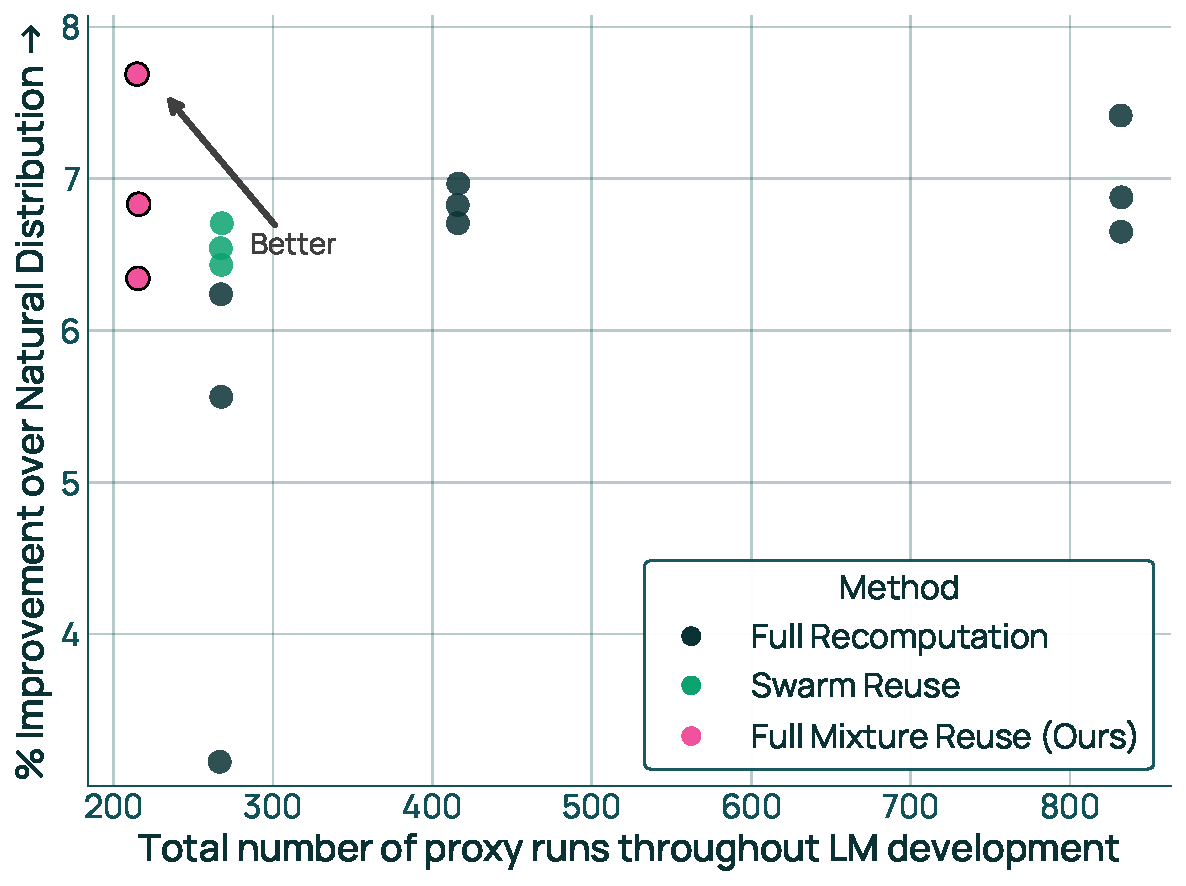
\includegraphics[width=0.5\linewidth]{figs/contribution_2/superswarm_6T.pdf}
    \caption{Performance improvement versus cost of mixing under evolving domains. \fullmixreuse achieves $99\%$ of the improvement of full recomputation while using $74\%$ fewer proxy runs.}
    \label{fig:superswarm_6T}
\end{figure}

\textbf{Low proxy run budget regime.} While Figure~\ref{fig:main_results} assesses performance versus number of proxy runs for cumulative costs ranging from 216 to 832 runs, it is unclear how recomputation strategies behave in a lower budget regime. We evaluate full recomputation with $c = 1$ (i.e., the minimum swarm size possible) and all other methods with $K \approx c(m+1)$ for $c = 1, 2, 3$, such that the range of total proxy runs considered is from 76 to 272.

Figure~\ref{fig:low_budget} shows performance versus number of proxy runs in a low budget regime. We make three observations:
\begin{itemize}
    \item The performance of swarm reuse versus \fullmixreuse at low budgets is similar.
    \item While the minimum number of proxy runs needed for full recomputation is 267, mixture reuse and swarm reuse unlock a lower budget regime, requiring as little as 76 runs. These reuse strategies can be attractive to practitioners with strict compute budgets and large domain sets that undergo many updates.
    \item With only 76 runs, mixture reuse still achieves a $+9.6\%$ and $+5\%$ improvement over the natural distribution when $R=1$T and $6$T, respectively.
\end{itemize}


\begin{figure}
    \centering
    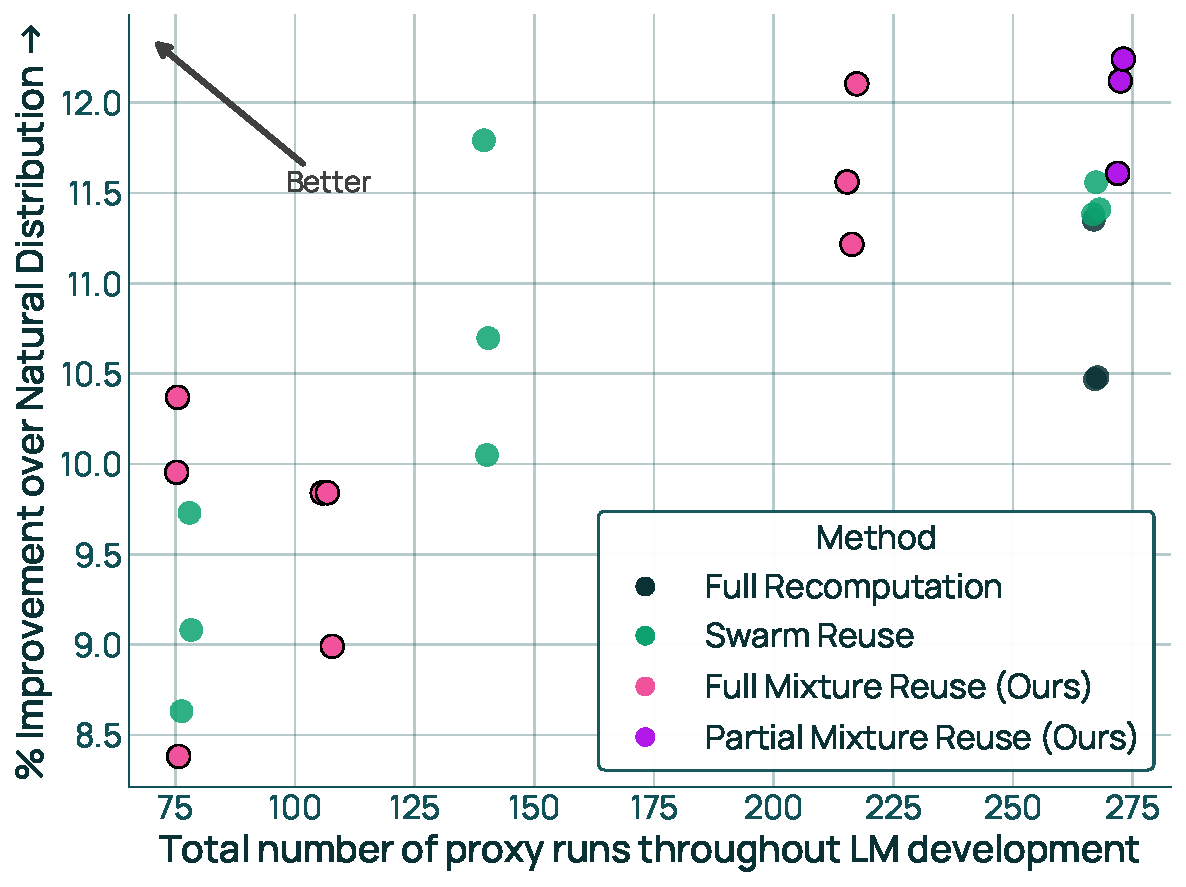
\includegraphics[width=0.49\linewidth]{figs/contribution_2/superswarm_1T_low_budget_regime.pdf}
    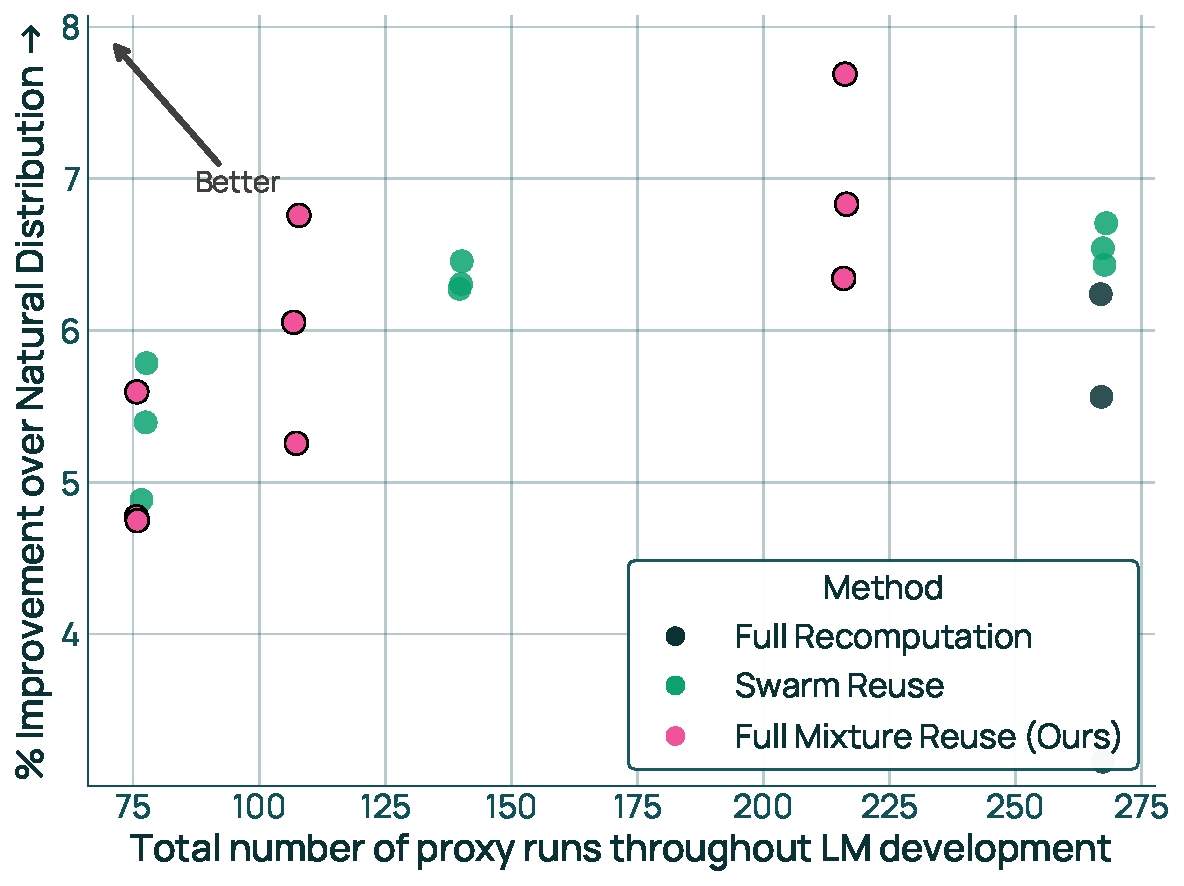
\includegraphics[width=0.49\linewidth]{figs/contribution_2/superswarm_6T_low_budget_regime.pdf}
    \caption{Performance improvement versus cost of mixing under evolving domains for $R=1$T (left) and $R=6$T (right). Total number of proxy runs vary from 76 to 272.}
    \label{fig:low_budget}
\end{figure}

\textbf{Proposed mixes.} Table~\ref{tab:full_domain_mixtures} shows the full mixtures corresponding to the natural distribution, full recomputation (best seed), and \partialmixreuse (best seed).

\begin{table}[t]
\centering
\caption{Mixture weights (full version of Figure~\ref{fig:superswarm_proposed_mixes}) for the natural distribution, full recomputation, and \partialmixreuse.}
\scriptsize
\setlength{\tabcolsep}{4pt}
\begin{tabular}{lccc | lccc}
\toprule
\textbf{Domain} & \textbf{Nat.} & \textbf{Full} & \textbf{Partial} & \textbf{Domain} & \textbf{Nat.} & \textbf{Full} & \textbf{Partial} \\
\midrule
arxiv & 0.003320 & 0.036555 & 0.022549 & pdf:fashion\_beauty & 0.000089 & 0.000003 & 0.000043 \\
dclm:adult\_content & 0.010828 & 0.006309 & 0.004050 & pdf:finance\_business & 0.009771 & 0.004230 & 0.001101 \\
dclm:art\_and\_design & 0.011291 & 0.006265 & 0.008097 & pdf:food\_dining & 0.000371 & 0.000113 & 0.009292 \\
dclm:crime\_and\_law & 0.027186 & 0.009991 & 0.005497 & pdf:games & 0.000397 & 0.000074 & 0.009944 \\
dclm:education\_and\_jobs & 0.029513 & 0.019003 & 0.008874 & pdf:health & 0.017292 & 0.013871 & 0.006251 \\
dclm:electronics\_and\_hardware & 0.012811 & 0.003289 & 0.003360 & pdf:home\_hobbies & 0.000627 & 0.000396 & 0.015698 \\
dclm:entertainment & 0.070592 & 0.055739 & 0.021609 & pdf:industrial & 0.004696 & 0.002512 & 0.000749 \\
dclm:fashion\_and\_beauty & 0.005953 & 0.003134 & 0.000769 & pdf:literature & 0.005095 & 0.005713 & 0.007648 \\
dclm:finance\_and\_business & 0.049587 & 0.022324 & 0.009896 & pdf:politics & 0.006269 & 0.001782 & 0.038680 \\
dclm:food\_and\_dining & 0.016928 & 0.015615 & 0.003785 & pdf:religion & 0.003952 & 0.001056 & 0.000088 \\
dclm:games & 0.036752 & 0.018811 & 0.013172 & pdf:science\_tech & 0.067792 & 0.029994 & 0.014598 \\
dclm:health & 0.062879 & 0.071471 & 0.050413 & pdf:software & 0.001462 & 0.001752 & 0.000000 \\
dclm:history\_and\_geography & 0.025735 & 0.028328 & 0.008994 & pdf:software\_dev & 0.006686 & 0.001929 & 0.015815 \\
dclm:home\_and\_hobbies & 0.020280 & 0.017861 & 0.005614 & pdf:sports\_fitness & 0.000871 & 0.000105 & 0.000060 \\
dclm:industrial & 0.006963 & 0.004541 & 0.007756 & pdf:transportation & 0.002740 & 0.001798 & 0.068597 \\
dclm:literature & 0.058299 & 0.048124 & 0.026746 & pdf:travel & 0.000336 & 0.000043 & 0.007881 \\
dclm:politics & 0.097667 & 0.034541 & 0.011652 & stack-edu:C & 0.000757 & 0.004088 & 0.001655 \\
dclm:religion & 0.044387 & 0.018381 & 0.006006 & stack-edu:CSharp & 0.001151 & 0.014910 & 0.015118 \\
dclm:science\_math\_and\_technology & 0.068254 & 0.077043 & 0.088744 & stack-edu:Cpp & 0.002002 & 0.012993 & 0.036761 \\
dclm:social\_life & 0.034952 & 0.018543 & 0.011095 & stack-edu:Go & 0.000223 & 0.003558 & 0.004103 \\
dclm:software & 0.017264 & 0.003887 & 0.002666 & stack-edu:Java & 0.005009 & 0.015251 & 0.025259 \\
dclm:software\_development & 0.035696 & 0.018979 & 0.025232 & stack-edu:JavaScript & 0.001420 & 0.004582 & 0.026072 \\
dclm:sports\_and\_fitness & 0.031441 & 0.017050 & 0.006516 & stack-edu:Markdown & 0.004621 & 0.028525 & 0.084832 \\
dclm:transportation & 0.014508 & 0.006398 & 0.003515 & stack-edu:PHP & 0.001182 & 0.003491 & 0.007554 \\
dclm:travel\_and\_tourism & 0.009211 & 0.005433 & 0.001804 & stack-edu:Python & 0.002879 & 0.072071 & 0.052859 \\
finemath-3plus & 0.005442 & 0.136232 & 0.136232 & stack-edu:Ruby & 0.000222 & 0.000868 & 0.004068 \\
pes2o & 0.009356 & 0.012147 & 0.006478 & stack-edu:Rust & 0.000227 & 0.000008 & 0.004161 \\
pdf:adult & 0.000048 & 0.000907 & 0.000016 & stack-edu:SQL & 0.001129 & 0.001833 & 0.002143 \\
pdf:art\_design & 0.001092 & 0.000231 & 0.004289 & stack-edu:Shell & 0.000406 & 0.008734 & 0.007459 \\
pdf:crime\_law & 0.006797 & 0.002672 & 0.000038 & stack-edu:Swift & 0.000241 & 0.006040 & 0.004430 \\
pdf:education\_jobs & 0.022072 & 0.010150 & 0.005608 & stack-edu:TypeScript & 0.000399 & 0.009983 & 0.001015 \\
pdf:entertainment & 0.000970 & 0.000087 & 0.003318 & wikipedia & 0.001609 & 0.017654 & 0.011671 \\
\bottomrule
\end{tabular}
\label{tab:full_domain_mixtures}
\end{table}



\textbf{Ablations for each domain update operator.} We demonstrate that \fullmixreuse attains performance similar to full recomputation for each type of domain update operator. We evaluate the following domain updates:
\begin{itemize}
    \item \Add: we start with 24 DCLM topic-based domains. Then, we add 15 Stack-Edu programming language domains.
    \item \Remove: we start with 39 domains consisting of 24 DCLM topics and 15 Stack-Edu programming languages. Then, we remove the 15 Stack-Edu domains.
    \item \Partition: we start with 24 DCLM topics and a single Stack-Edu source domain. Then, we partition the Stack-Edu source into 15 programming language domains. 
    \item \Revise: we start with 24 DCLM topics and a single StackV2~\citep{lozhkov2024starcoder} source domain. Then, the StackV2 domain is replaced with the Stack-Edu domain.
\end{itemize}

For each operator, we compare \fullmixreuse and the natural distribution over $\D'$ (as a control) against full recomputation. We measure the total variation distance of the proposed mixtures with respect to full recomputation's mix, defined as $\tv(q, q^\star) = \frac{1}{2} \sum_{i=1}^{m'} |q_i - q_i^\star| \in [0, 1]$. We also measure performance gap relative to full recomputation's downstream performance (average task BPB) for \Add, \Remove, and \Partition. For our setup, we used $k=4$, $R=6$T.


Figure~\ref{fig:operators} shows that \fullmixreuse achieves substantially smaller performance gaps and TV distances compared to the natural distribution across \Add, \Remove, and \Partition. For \Revise, the TV distance between \fullmixreuse and full recomputation was only 0.21\%---orders of magnitude smaller than other operators---indicating nearly identical mixes. We therefore did not evaluate downstream performance for \Revise, as variation would be dominated by noise. These results demonstrate that mixture reuse works effectively across all domain update operators.


\begin{figure}
    \centering
    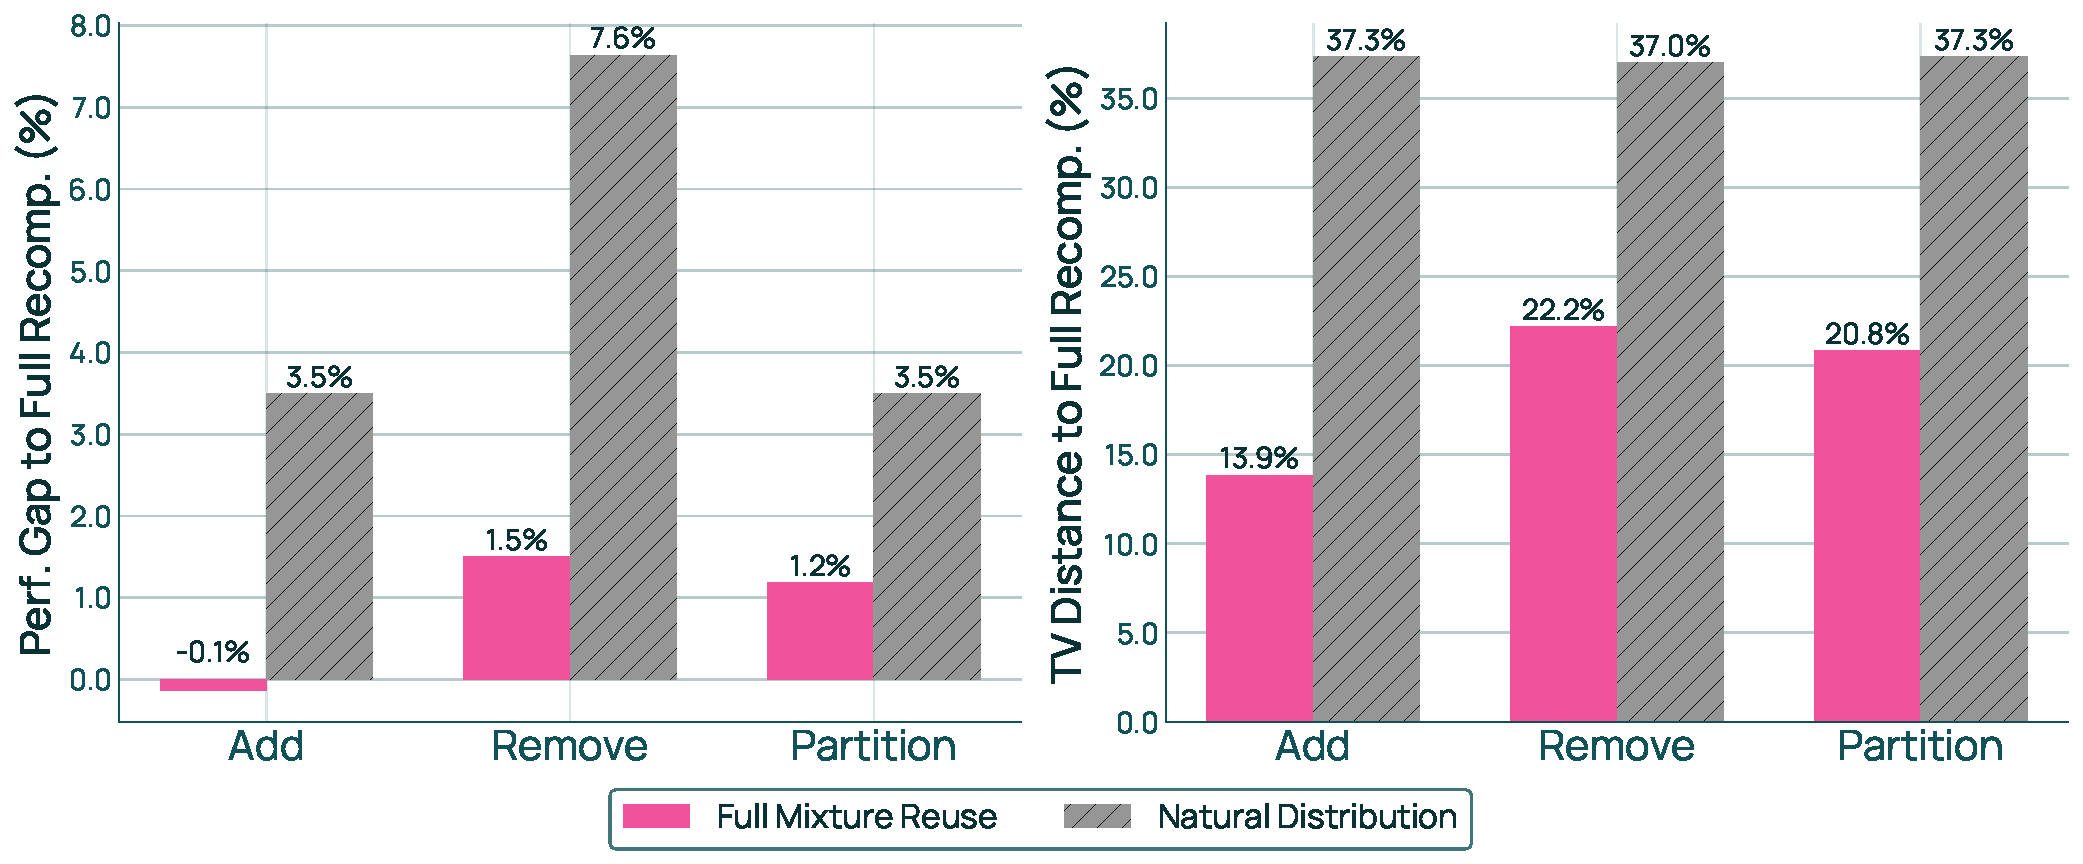
\includegraphics[width=\linewidth]{figs/contribution_2/operator_fig.pdf}
    \caption{Relative performance gap (left) and total variation distance (right) w.r.t. full recomputation across domain update operators. \fullmixreuse is substantially closer to full recomputation than the natural distribution across all three operators, in both performance and mixes.}
    \label{fig:operators}
\end{figure}




